\documentclass{VUMIFPSbakalaurinis}
\usepackage{algorithmicx}
\usepackage{algorithm}
\usepackage{algpseudocode}
\usepackage{amsfonts}
\usepackage{amsmath}
\usepackage{bm}
\usepackage{caption}
\usepackage{color}
\usepackage{float}
\usepackage{graphicx}
\usepackage{listings}
\usepackage{subfig}
\usepackage{wrapfig}
\usepackage{listings}

\lstset {
  language=Scala,
  basicstyle=\footnotesize,
  numbers=left,
  stepnumber=1,
  showstringspaces=false,
  tabsize=1,
  breaklines=true,
  breakatwhitespace=false,
}

% Titulinio aprašas
\university{Vilniaus universitetas}
\faculty{Matematikos ir informatikos fakultetas}
\institute{Informatikos institutas}  % Užkomentavus šią eilutę - institutas neįtraukiamas į titulinį
\department{Programų sistemų bakalauro studijų programa}
\papertype{Bakalauro baigiamasis darbas}
\title{Translation Unit Granularization}
\titleineng{Kompiliatoriaus transliuojamo vieneto smulkinimas}
\author{Andrius Bentkus}
% \secondauthor{Vardonis Pavardonis}   % Pridėti antrą autorių
\supervisor{asist. dr. Vytautas Valaitis}
\reviewer{doc. dr. Vardauskas Pavardauskas}
\date{Vilnius – \the\year}

% Nustatymai
% \setmainfont{Palemonas}   % Pakeisti teksto šriftą į Palemonas (turi būti įdiegtas sistemoje)
\bibliography{bibliografija}

\begin{document}
\maketitle

%% Padėkų skyrius
% \sectionnonumnocontent{}
% \vspace{7cm}
% \begin{center}
%     Padėkos asmenims ir/ar organizacijoms
% \end{center}

\sectionnonumnocontent{Summary}
This thesis presents an approach on how to speed up compilation in a day to day programming scenario, benchmarks the performance improvements with various inputs and compares the gathered performance metrics to an already existing compiler.

Classic compilers treat a source file as an atomic translation unit in their compilation pipeline, the proposed approach tries to leverage the structure of modern programming languages to granularize the translation unit in order to improve recompilation times for classic development workloads.

The chosen target language is a subset of the Scala programming language.
Instead of modifying the standard Scala compiler to accomodate the proposed approach, a compiler is written from scratch in order to have simple program enabling straigtforward modifications for an easier accomodation of the proposed approach.

Performance measurements of the prototype compiler are taken with the approach enabled and disabled, various dynamic inputs are generated with different compilation unit sizes to gain insights in the effectivness of the approach.
Results are then compared to the classic compiler and conclusions are drawn.

\keywords{Compilers, Translation Unit, Compiler optimization}

\sectionnonumnocontent{Santrauka}
% TODO: translation in lithuanian

% Nurodomi iki 5 svarbiausių temos raktinių žodžių (terminų).
% Vienas terminas gali susidėti iš kelių žodžių.
\raktiniaizodziai{Transliavimas, Transliavimo optimizacijos}


\tableofcontents

\sectionnonum{Introduction}

\subsectionnonum{Overview}
\subsectionnonum{Contributions}
\subsectionnonum{Outline}

\section{Optimization}
\subsection{Translation Unit}
The classic aproach of compilers is to read an entire source file and generate a corresponding output file with the translated code.

For example in C++ and C source files with the extensions .cpp or .c are compiled to an intermediate object file with the extension .o, containing the generated assembly code of a specific target architecture, x86, ARM, etc.
Once all source files are compiled into object files, all object files are combined together with optional resources into a singular output file called the executable.

The Java language forces the programmer to define every Java class in its own file and every .java file is then compiled to a .class file, which can be later packaged to .jar files together with additional resources for easier deployment.
A .class file contains all the Java bytecode generated from the Java source file, a condensed representation of the a Java class in a high level format which is abstract and does not target any specific target architecture, but an abstract architecture called the Java Virtual Machine (JVM).
Code targeting the JVM can be then executed provided a Java runtime is present on the target machine which Just in Time (JIT) compiles the bytecode to the target machines assembly code and executes it.

% todo: maybe later?
Java bytecode is much more abstract and conceptually closer to the original representation of a class than the generated object files containing assembly are.
Java class methods are basically sections in a .class file \cite{JvmMethods} which wrap Java bytecode - the implementation of the methods functionality.
This high level representation makes granularization of translation units much more convient, because it is possible to map a method directly to an entire section within the class file.

Scala also targets the JVM, however it does not share the limitation of one class per source file that Java has.
A Scala source file can contain multiple class definitions in a singular and due to the possibility to define class in a very concise manner developers gravitate towards multiple class definitions per file \ref{multidef}.

% listings https://tex.stackexchange.com/questions/321843/using-labels-for-lstinputlisting

\lstinputlisting[language=Scala, linewidth=18cm, label={multidef}, caption={An interface and 3 class definitions in a singular source file}]{./code/Expression.scala}

The compiler creates in total 4 corresponding .class files as depicted in Listing \ref{img:Expression}.
The classes all depend on the same trait definition called Expression, which is an empty interface in Java called a Marker Interface \cite{10.5555/1407381}, however there is no need for a strict compilation order, the compiler can utilize the meta information to compile all result .class files in parallel or whatever order it sees fit.

When running the compiler with the source file displayed in \ref{multidef} as the input, the compiler will recompile all 4 classes, even though new modifications might be present only within one class because the minimal translation unit is the entire source file.
In the given examples the classes are trivial and the performance when recompiling is negligible.

\begin{figure}[H]
    \centering
    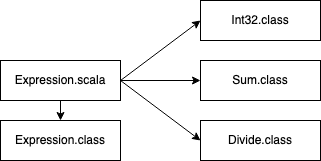
\includegraphics[scale=0.6]{img/Expression}
    \caption{Compilation result of Listing \ref{multidef}}
    \label{img:Expression}
\end{figure}

One might argue that multiple sizeable class implementations with numerous methods contained in a singular source file are rare in actual code bases and optimizing for this case would yield miniscule benefits outside of tailored benchmarks, but the opposite is the truth. % todo: replace but a the opposite is true.
In the following example a rather standard usage of the unit testing library specs2 is shown.

\sectionnonum{Results and conclusion}
\subsectionnonum{Results}
This is the result.

\printbibliography[heading=bibintoc]  % Šaltinių sąraše nurodoma panaudota
% literatūra, kitokie šaltiniai. Abėcėlės tvarka išdėstomi darbe panaudotų
% (cituotų, perfrazuotų ar bent paminėtų) mokslo leidinių, kitokių publikacijų
% bibliografiniai aprašai. Šaltinių sąrašas spausdinamas iš naujo puslapio.
% Aprašai pateikiami netransliteruoti. Šaltinių sąraše negali būti tokių
% šaltinių, kurie nebuvo paminėti tekste. Šaltinių sąraše rekomenduojame
% necituoti savo kursinio darbo, nes tai nėra oficialus literatūros šaltinis.
% Jei tokių nuorodų reikia, pateikti jas tekste.

% \sectionnonum{Sąvokų apibrėžimai}
\sectionnonum{Acronyms}

\textbf{AST} - Abstract Syntax Tree

\textbf{JVM} - Java Virtual Machine

\textbf{JIT} - Just In Time

\appendix  % Priedai
% Prieduose gali būti pateikiama pagalbinė, ypač darbo autoriaus savarankiškai
% parengta, medžiaga. Savarankiški priedai gali būti pateikiami ir
% kompaktiniame diske. Priedai taip pat numeruojami ir vadinami. Darbo tekstas
% su priedais susiejamas nuorodomis.

\section{Neuroninio tinklo struktūra}
\begin{figure}[H]
    \centering
    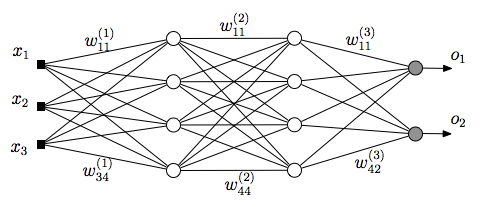
\includegraphics[scale=0.5]{img/MLP}
    \caption{Paveikslėlio pavyzdys}
    \label{img:mlp}
\end{figure}


\section{Eksperimentinio palyginimo rezultatai}
% tablesgenerator.com - converts calculators (e.g. excel) tables to LaTeX
\begin{table}[H]\footnotesize
  \centering
  \caption{Lentelės pavyzdys}
  {\begin{tabular}{|l|c|c|} \hline
    Algoritmas & $\bar{x}$ & $\sigma^{2}$ \\
    \hline
    Algoritmas A  & 1.6335    & 0.5584       \\
    Algoritmas B  & 1.7395    & 0.5647       \\
    \hline
  \end{tabular}}
  \label{tab:table example}
\end{table}

\end{document}
